\documentclass[11pt]{article}

%FOR SCRIBES: Please change the next three lines to reflect the correct
%FOR SCRIBES: lecture number, name, and date.
\newcommand{\lecturenumber}{1-3}
%\newcommand{\scribename}{Phillip Janowski}
\newcommand{\lecturedate}{8/24 - 8/28} 

%\usepackage{subfigure}
\usepackage{color}
\usepackage{url}
\usepackage{graphicx}
\usepackage{fullpage}
\newcommand{\etal}{{\em et al.}}
\newcommand{\qed}{\mbox{}\hspace*{\fill}\nolinebreak\mbox{$\rule{0.6em}{0.6em}$}}
\newcommand{\expect}{{\bf \mbox{\bf E}}}
\newcommand{\var}{{\bf \mbox{\bf Var}}}
\newcommand{\prob}{{\bf \mbox{\bf Pr}}}
\newcommand{\ntt}{n^{3/4}}
\usepackage[english,portuguese]{babel}
\addto\captionsportuguese{\renewcommand{\figurename}{Fig.}}
\addto\captionsportuguese{\renewcommand{\refname}{References and Further Reading}}

%--------------------------- Commands and Environments I added -----------------
\usepackage[english]{babel}
\usepackage{amssymb,hyperref}
\usepackage{amsmath}
\usepackage{array, fancyhdr, bm, listings}
\usepackage{algorithm,comment}
\usepackage{algorithmic}
\usepackage{subcaption}
\usepackage{thmtools, thm-restate}
\usepackage{fancyhdr,mathtools}
\renewcommand{\baselinestretch}{1.10}
\DeclarePairedDelimiter\set\{\}
%%      Fonts:
%%---------------------------------------------------------------------------
\newfont{\bssten}{cmssbx10}
\newfont{\bssnine}{cmssbx10 scaled 900}
\newfont{\bssdoz}{cmssbx10 scaled 1200}

%---------------------------------------------------------------------------
\newcounter{topic} \setcounter{topic}{0}
\newcommand{\topic}[1]{\par \refstepcounter{topic} {\bssdoz \arabic{topic}.~ #1} \par}
%\newcommand{\topic}[1]{\par \refstepcounter{topic} \vs{2ex} {\bssdoz \arabic{topic}.~ #1} \par \vs{1ex}}

%------------------------------ end of new commands and evironments ------------

\definecolor{gray}{rgb}{0.5,0.5,0.5}
%\newcommand{\comment}[1]{{\color{gray}[\textsf{#1}]}}
\newcommand{\redospace}{\small\renewcommand{\baselinestretch}{1.5}\normalsize}
\newcommand{\undospace}{\small\renewcommand{\baselinestretch}{1}\normalsize}
\newtheorem{theorem}{Theorem}[section]
\newtheorem{lemma}[theorem]{Lemma}
%----------------------------- some other things I added ---------------------
\newtheorem{claim}[theorem]{Claim}
\newtheorem{example}[theorem]{Example}
\newtheorem{protocol}[theorem]{Protocol}
%----------------------------------------------------------------------------
\newtheorem{corollary}[theorem]{Corollary}
\newtheorem{definition}{Definition}[section]
\newtheorem{remark}[definition]{Remark}
\newtheorem{conjecture}[theorem]{Conjecture}
\newtheorem{proposition}[theorem]{Proposition}
\newenvironment{proof}{{\bf Proof:}}{$\qed$\par}
\newenvironment{proofof}[1]{{\bf Proof of #1:}}{$\qed$\par}
\newenvironment{proofsketch}{{\sc{Proof Outline:}}}{$\qed$\par}

\usepackage{hyperref}
\hypersetup{
bookmarksnumbered
}

\begin{document}
\begin{center}
\framebox{\parbox{6.5in}{
{\bf{CS 5001/6001: Intro to Quantum Computing\hfill Spring 2021}}\\
%\href{https://www.avahbanerjee.com/cs6200.html}{https://www.avahbanerjee.com/cs6200.html}\\ 
Group Members:
Phill Janowski, Md Yasin Kabir \\\
%{\bf Lectures:  \lecturenumber \hfill Dates: \lecturedate}
}}
\ \\
\end{center}
%\setcounter{section}{\lecturenumber}
%FOR SCRIBES: ---------- Begin Scribing Here ------------------------

\section{The Problem and the Algorithm}

We sought to find the minimum value of a list of numbers while using the fewest amount of queries checking that the value was the minimum value. Grover's Search Algorithm allows us to make a query to a function with multiple to values which then returns true or false whether the values as valid to the function or not. The function resides in an the oracle that marks the values of values that the function returns true for. The rest of the circuit amplifies those marked values. We are able to send the oracle all the possible values by superimposing them onto each other. We designed an function generator that creates a boolean function that should return true if the binary value of an index is passed in in binary form satisfies the conditions we choose. In our case our condition is if the index of some list L corresponding to the input value is greater than the current lowest value we have found in index y of L, or L[n] $\textless$  L[y]. The boolean value will be returned from the function and used to determine whether or not the sign on the statevector that represents the index of the list we are checking is flipped by the oracle. If the return value is true, the sign will be flipped, marking the value as a valid state, else it remains the same. The Grover algorithm then flips all of the states across the axis of the superposition of inputs, making the states we want to show as valid that are negative positive states with a much greater amplitude than the invalid states that are still sitting at the same uniform superposition amplitude.

To test the implementation, we generated a random list of numbers, L, and pick a starting index, y, at random. If after an iteration of the circuit, the top measured value of the circuit represents an index of L that holds a smaller value than y, then we use the top measured value as our y for the next iteration of the circuit. In simpler terms, if the measured value of the circuit is y' and L[y'] $\textless$ L[y], then y = y'. The boolean function is regenerated, and consequently the oracle, with the new value of y in mind and the circuit is recreated with the new oracle. This continues for a set amount of iterations, m, that should be optimized for our set of parameters to solve this problem in the least amount of iterations.

\section{Circuit Design}

The Grover's algorithm part of our circuit was mostly handle by Qiskit, using their canned Grover operator to wrap an oracle that we provided. The operator begins by placing Hadamard gates on every qbit, creating a superposition of all states. The states then pass into one of two oracles that are implemented and in various states of working, however both use the same algorithm to generate the function for the oracle.

The most working implementation is using a Qiskit Logical Expression Oracle that takes in a boolean expression such as
(not a \& b \& not c \& d) or ( not a \& b \& not c \& not d)
to determine the validity of the state that is currently on the circuit in relation to the L[n] $\textless$ L[y] condition we set. The boolean expression is generated before every run of the circuit because if the algorithm has not found the correct value and the circuit is working as expected, the value of y should have changed and the boolean expression will have fewer possible inputs that will satisfy it. The expression is eventually whittled down one expression that is only satisfied by the index value of L that contains the smallest value in the list.

The other implementation, using a Qiskit Custom Circuit Oracle, works almost identically, except when it is used in conjunction with the Grover algorithm implementation in Qiskit, it fails to flip the sign on any state. From the boolean function generator that is used with the logical expression oracle, we create a boolean function that is provided as a callback function to the oracle. The callback function takes in the bits that are provided by the circuit and are then placed in the boolean expression and evaluated. The result of the evaluation is returned along with the every input after the first xor'd with the return value to make the circuit reversible. If we call the result of the evaluated expression 'result' and the input to the oracle is w, x, y, and z, then the output of the oracle would be [result, result $\oplus$ x, result $\oplus$ y, result $\oplus$ z]

The results of the are taken out superposition by applying Hadamard gates again to the qbits and the marked states are returned with higher amplitudes than the non marked states.

\\\
\\\
\\\
\begin{center}
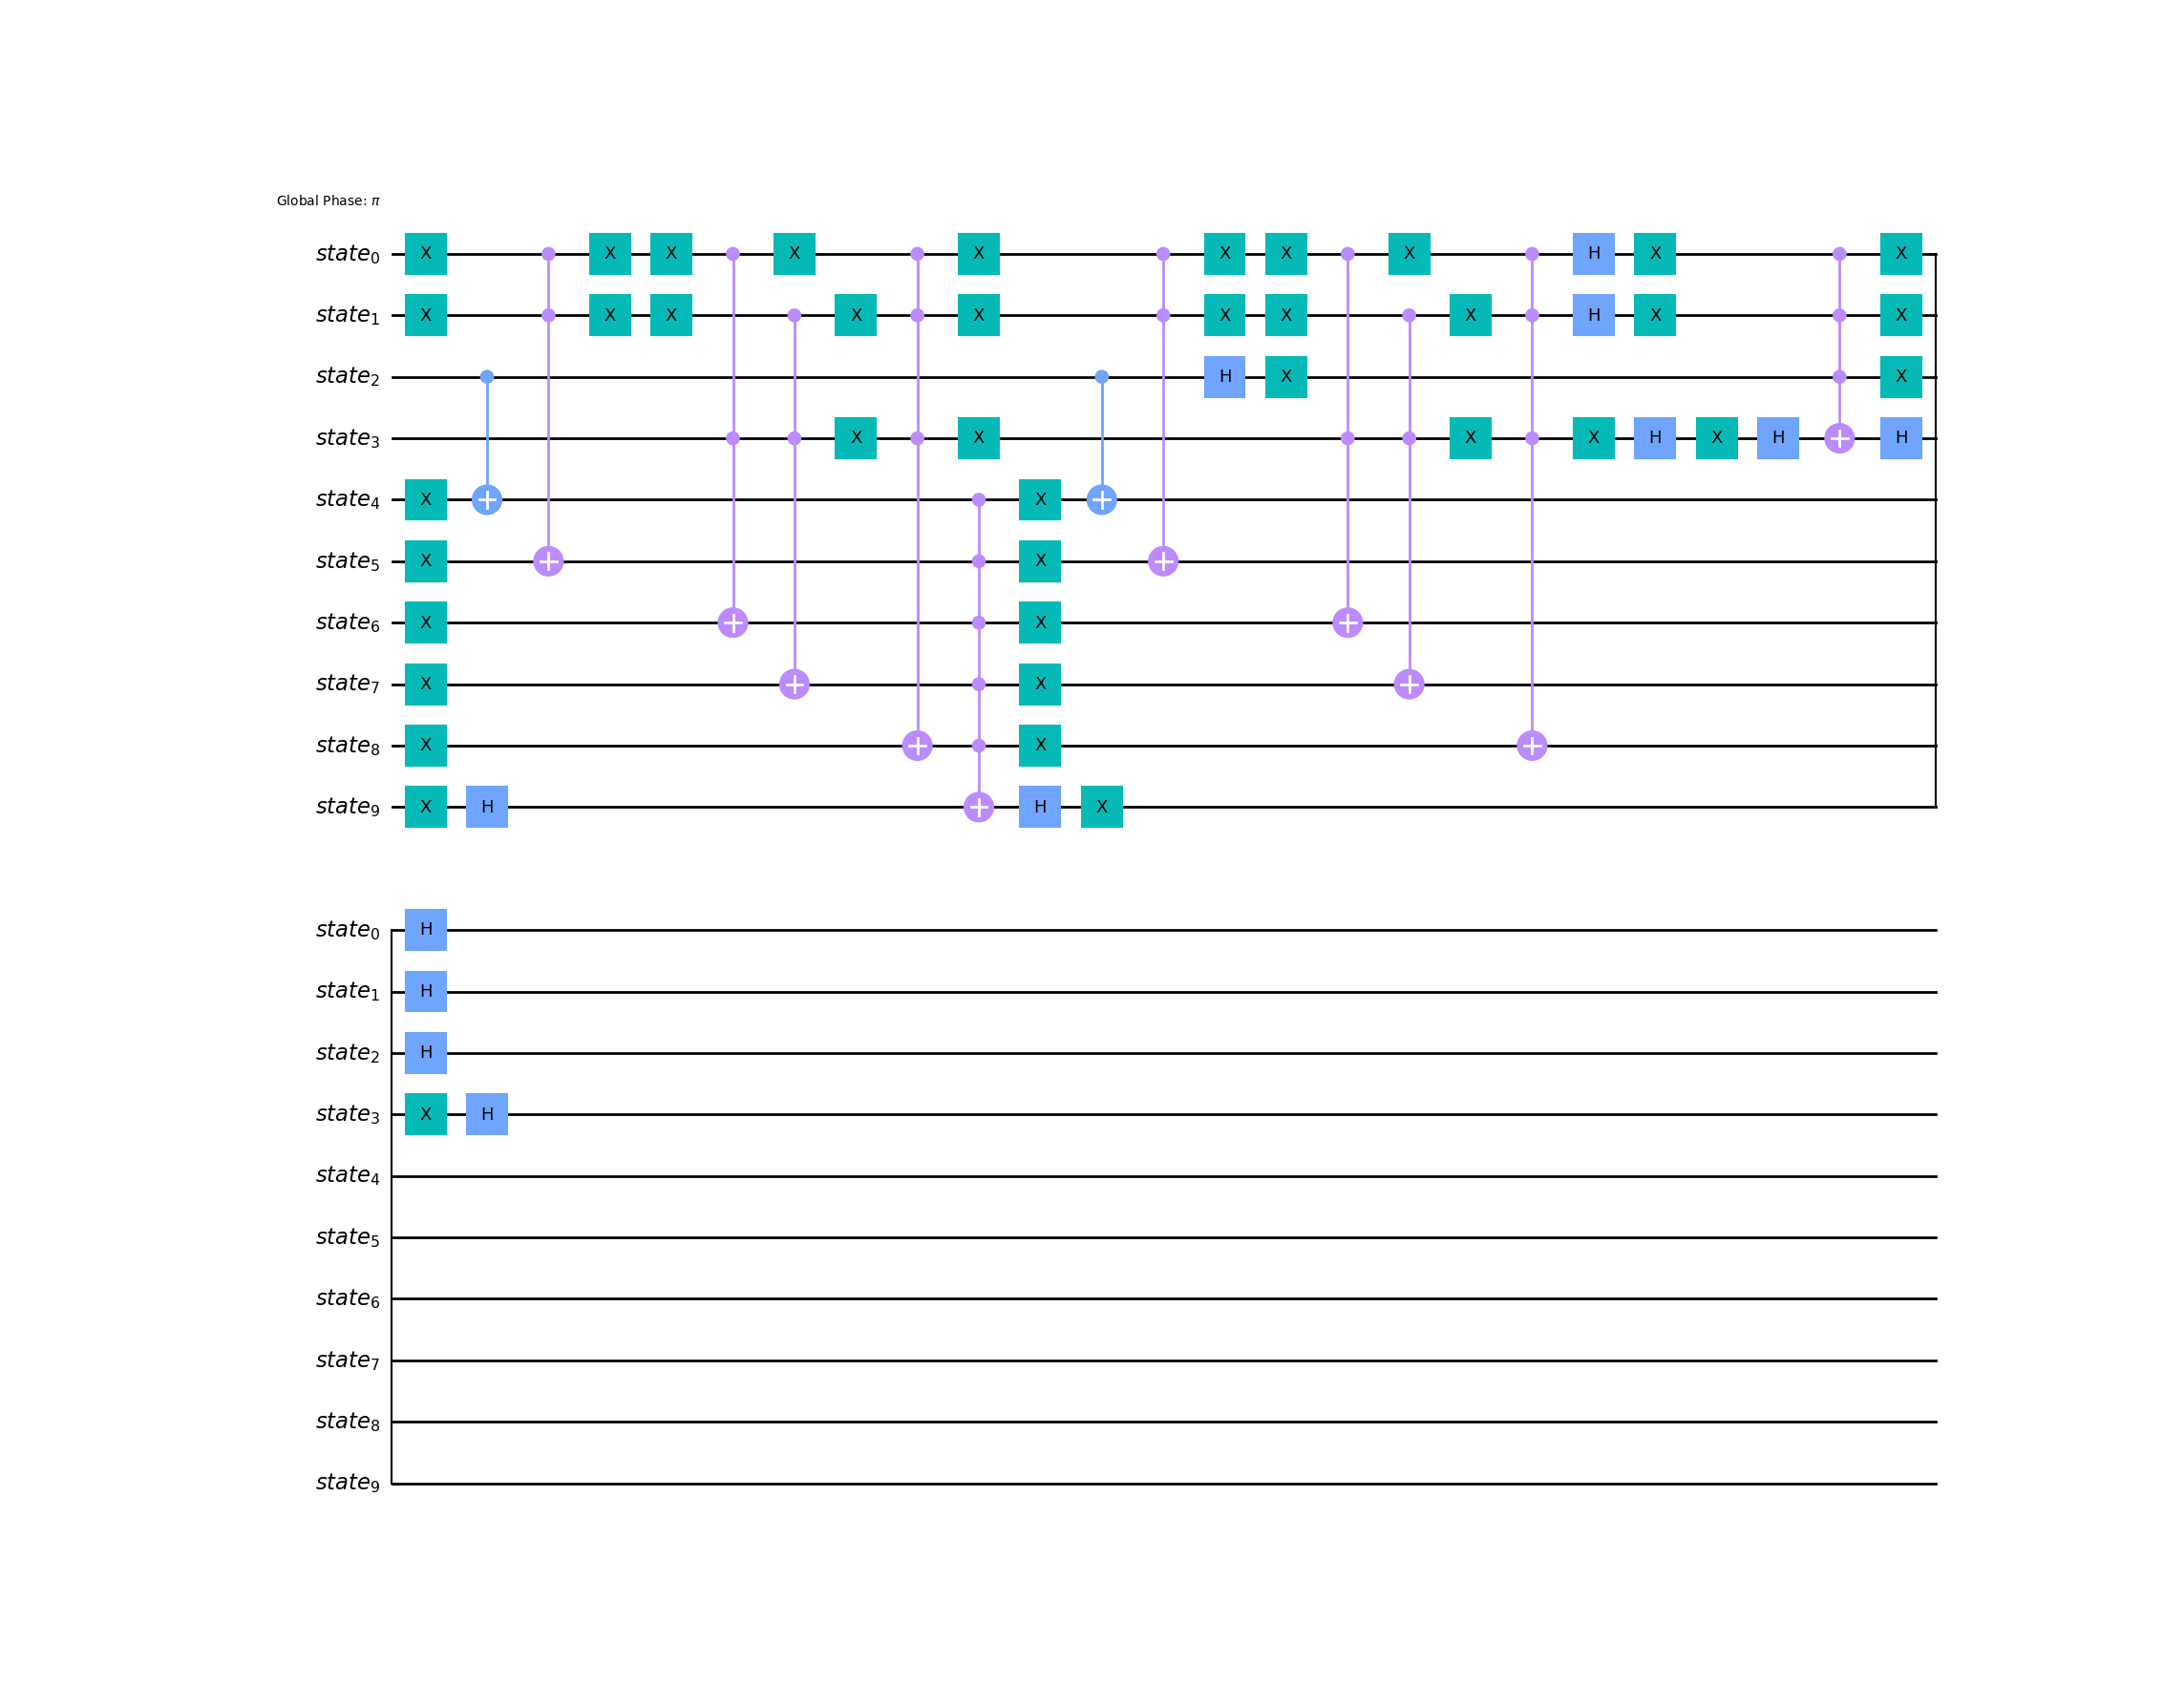
\includegraphics[width=\textwidth]{logical_expression_grover.png}
A generated circuit using the Logical Expression Oracle. This is generated using the logical expression that is processed and used to construct the circuit and then wrapped by the standard Grover circuit.
\end{center}

\begin{center}

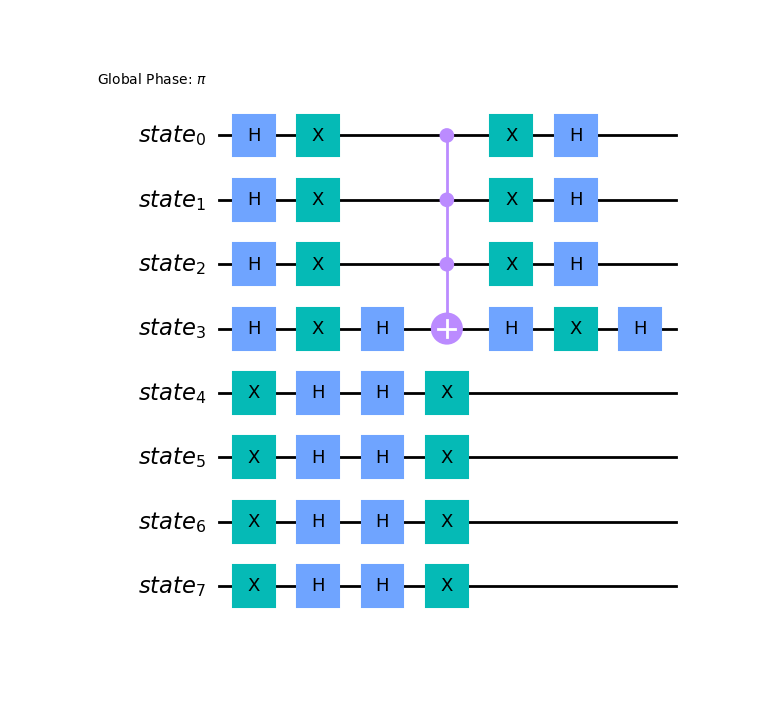
\includegraphics[width=\textwidth]{custom_circuit_grover.png}
A generated circuit using the Custom Circuit Oracle. This is generated and displays only as the standard Grover circuit without the oracle. The logic from the generated callback function is not shown here.
\end{center}

\newpage

\section{Experiments}

Experimenting with these circuits proved difficult given that one circuit, the Logical Expression Oracle circuit worked and marked the correct states some of the time and the Custom Circuit Oracle never marked anything.

A pattern arose from the circuit running with the logical expression oracle. Proper states were getting marked sometimes and if they weren't, the reversed bit string of the proper states were. For example, if the oracle should have marked the value 1 (state 0001) as valid, the value 8 (state 1000) would be marked. Logs would show that there wasn't a valid boolean expression for 1000 to make it return true. This became clearer the more tests that were run as only the indexes with symmetrical binary values that held the smallest value, such as 6 represented by 0110, were the only times that the algorithm would successfully find the smallest valued index. Creating logs that output the values of the reversed values of the marked states showed this to be a very common occurrence. Unit tests were written for the generation and evaluation functions that were being used that proved that the functions were behaving as they were expected to be.


A similar issue around what seemed to be the black box of the Grover circuit creator provided by Qiskit was evident with runs using the Custom Circuit Oracle. As previously stated, circuits created with this oracle did not mark any states. However, the callback function provided to this oracle was being hit and was returning the correct values, the grover operator was just refusing to acknowledge them.


Different m values were used, m being the number of attempts given to find the index of the smallest value in the list L. This did not seem to affect the number of times that the logical expression gate was successful but it seem to help the custom circuit oracle come up with the correct value. This is definitely because the value picked for the custom circuit oracle circuit was much more random since no state was ever marked, so the more runs it had the more likely it was to end up with an index of L as the top measurement that was less than the current L[y]. m = 5 seemed to be as consistent for the logical expression oracle circuit as any other value.

\newpage
\begin{center}
Here are the histograms showing the marked states of the logical expression oracle circuit. This was from a successful run, log output is included at the end of the page. The L[y] values shows the smallest found value for that iteration. The value 0000 is marked after L[y] = 0 because that is the default case we included when there are no L[y] values smaller than the current L[y] value. This was to prevent the circuit from blowing up when trying to evaluate an empty expression.
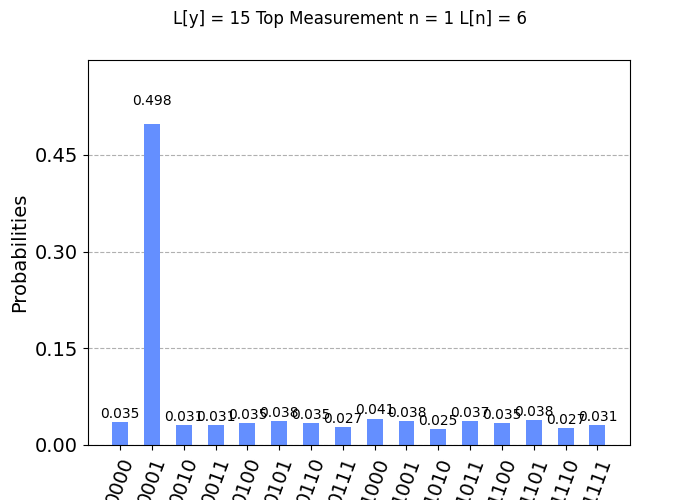
\includegraphics[width=\textwidth]{logical_0.png}

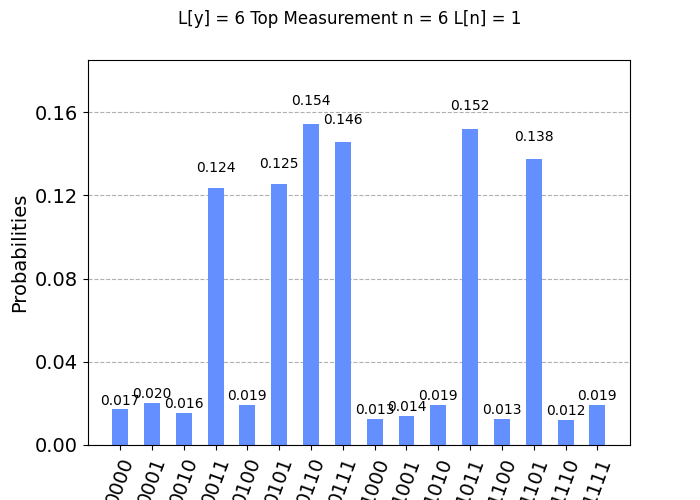
\includegraphics[width=\textwidth]{logical_1.png}

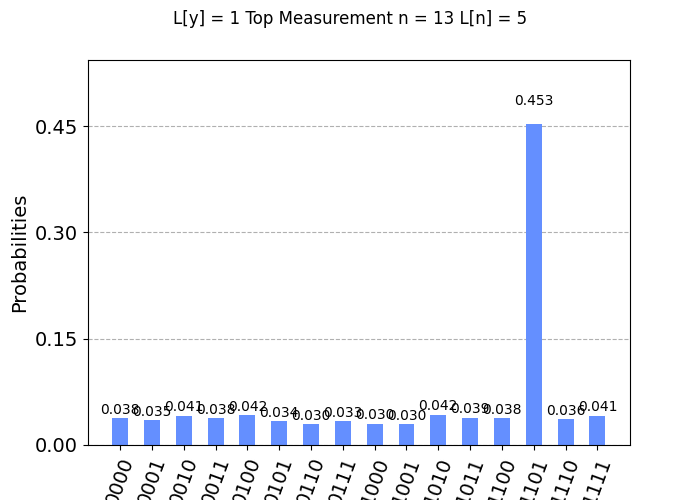
\includegraphics[width=\textwidth]{logical_2.png}

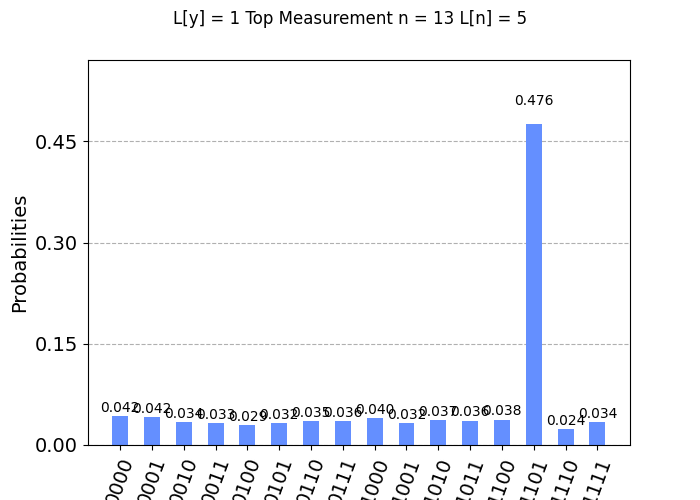
\includegraphics[width=\textwidth]{logical_3.png}

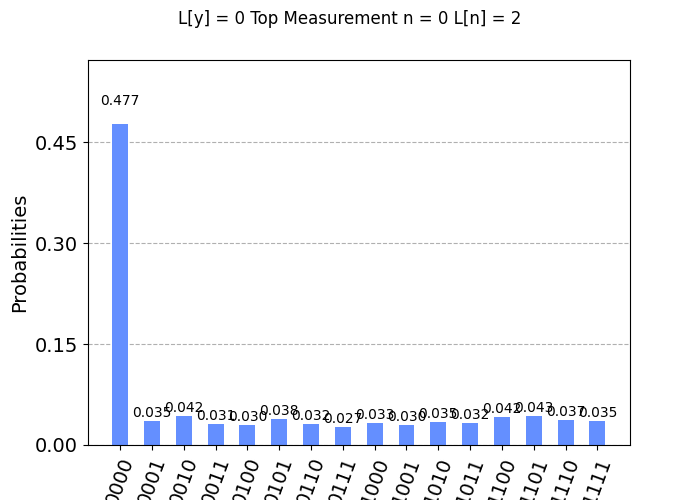
\includegraphics[width=\textwidth]{logical_4.png}
\end{center}

\newpage
\begin{center}
Here are the histograms showing the marked states of the logical expression oracle circuit from a failed run. For some reason, only the the number 15 was found in the list. Log output is also included for this run. In the log output you can see that there is a case in the logical expression for every value except for L[y] = 15.
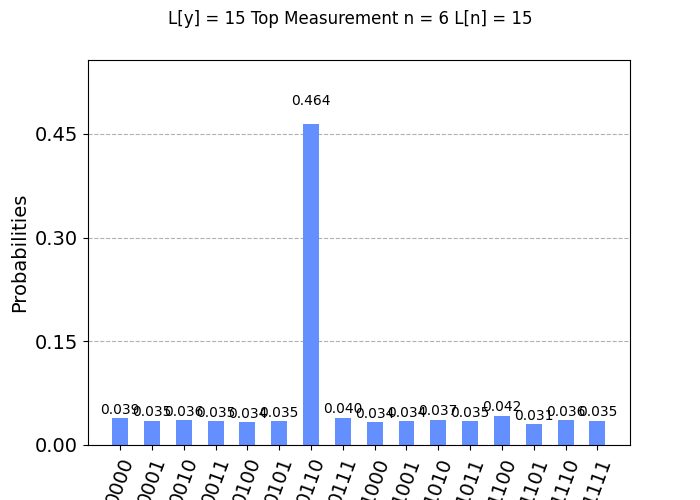
\includegraphics[width=\textwidth]{failed_logical_0.png}

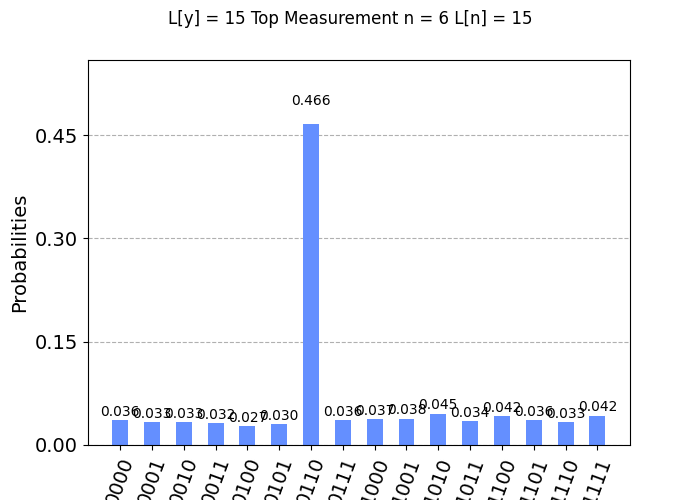
\includegraphics[width=\textwidth]{failed_logical_1.png}

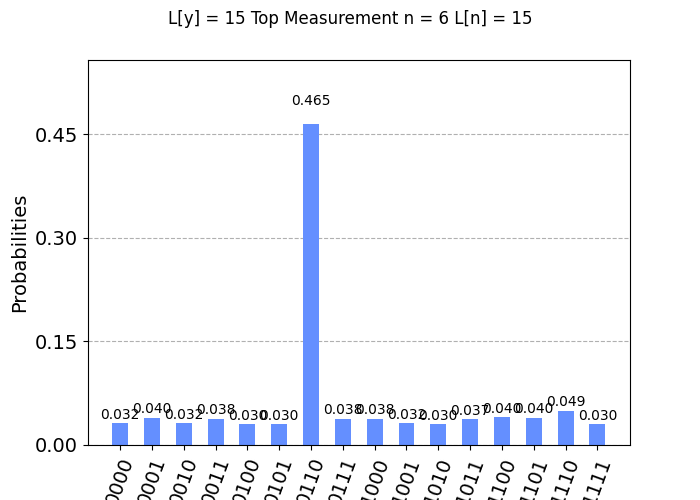
\includegraphics[width=\textwidth]{failed_logical_2.png}

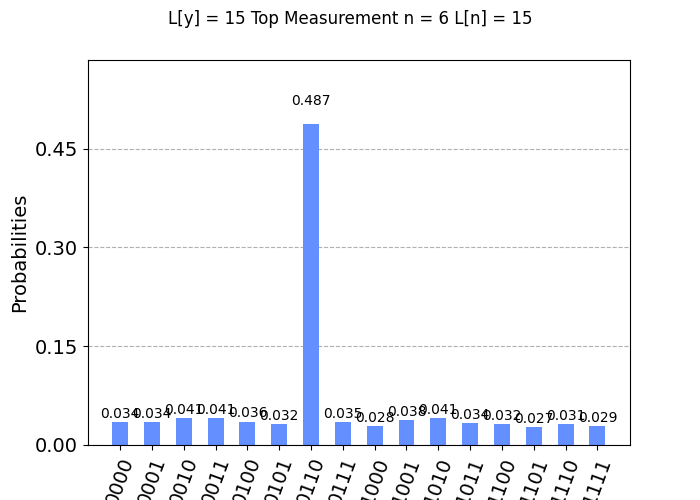
\includegraphics[width=\textwidth]{failed_logical_3.png}

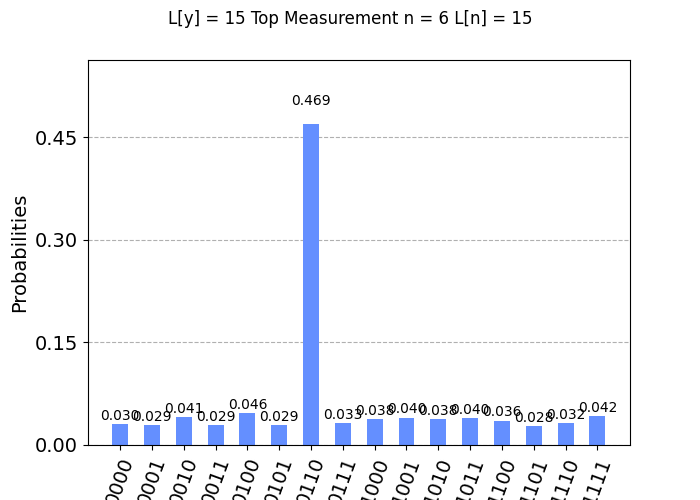
\includegraphics[width=\textwidth]{failed_logical_4.png}
\end{center}

\newpage
\begin{center}
Here are the graphs showing that all states are unmarked when using the custom circuit oracle. Note that non are getting marked yet the correct.
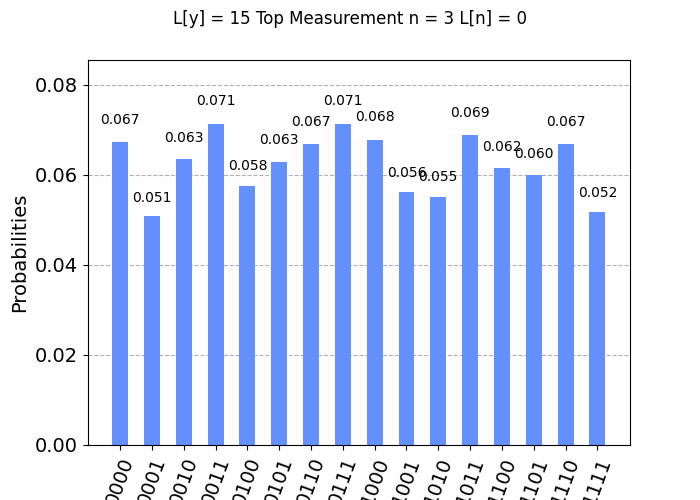
\includegraphics[width=\textwidth]{custom_0.png}

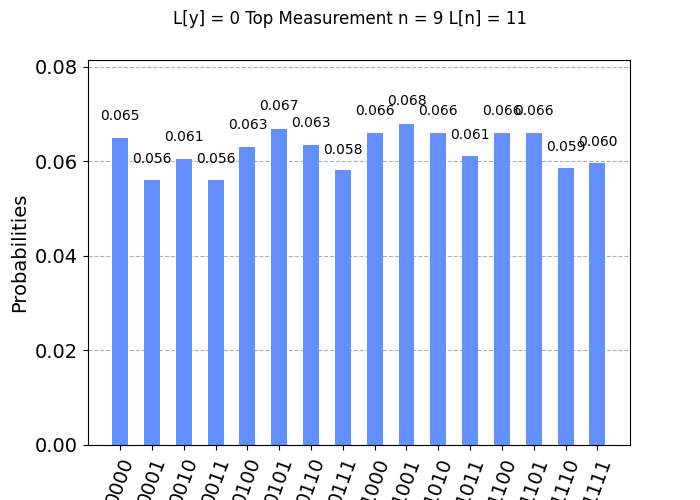
\includegraphics[width=\textwidth]{custom_1.png}

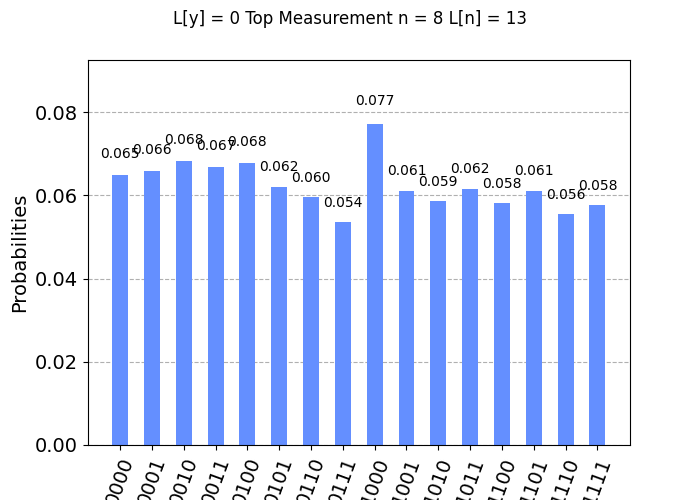
\includegraphics[width=\textwidth]{custom_2.png}

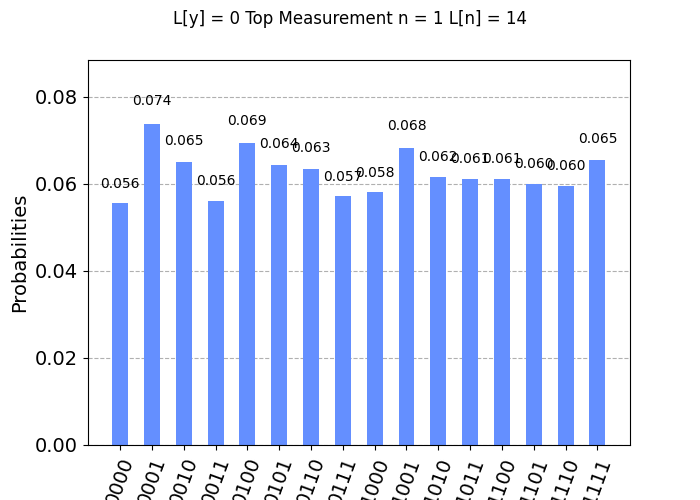
\includegraphics[width=\textwidth]{custom_3.png}

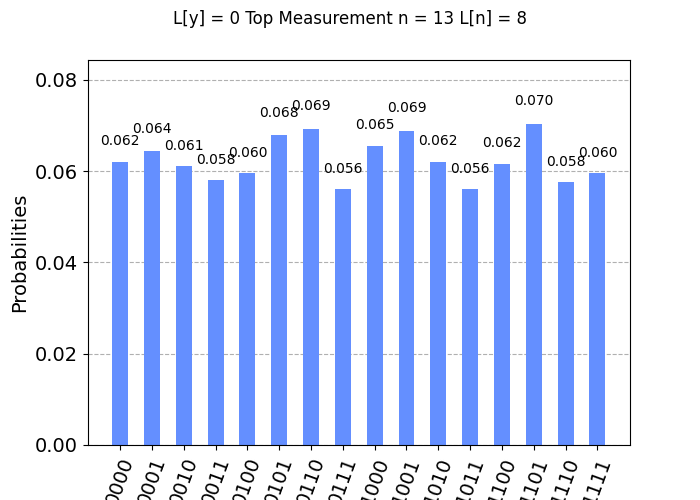
\includegraphics[width=\textwidth]{custom_4.png}
\end{center}

\newpage
Here is the log output from a run of the logical expression circuit showing that the proper boolean functions and being run and evaluating correctly yet the proper states are not being marked. The format for the 'all measurements' is as follows, '6': (144, '0110', 7), '6' being the integer value of the state, '144' being the number of hits, '0110' being the bit value, and '7' being the L[6] value.

\begin{verbatim}
L = [2, 6, 0, 5, 12, 3, 1, 15, 14, 10, 9, 13, 4, 11, 8, 7]
index containing 0 = 2
y = 7 | 0111
L[y] = 15
truth table = ['1', '1', '1', '1', '1', '1', '1', '0', '1', '1', '1', '1', '1', '1', '1', '1']

Boolean Functions for Oracle
 (  ~a &  ~b &  ~c &  ~d )  clause for marking y=0 L[y]=2
 (  ~a &  ~b &  ~c & d )  clause for marking y=1 L[y]=6
 (  ~a &  ~b & c &  ~d )  clause for marking y=2 L[y]=0
 (  ~a &  ~b & c & d )  clause for marking y=3 L[y]=5
 (  ~a & b &  ~c &  ~d )  clause for marking y=4 L[y]=12
 (  ~a & b &  ~c & d )  clause for marking y=5 L[y]=3
 (  ~a & b & c &  ~d )  clause for marking y=6 L[y]=1
 ( a &  ~b &  ~c &  ~d )  clause for marking y=8 L[y]=14
 ( a &  ~b &  ~c & d )  clause for marking y=9 L[y]=10
 ( a &  ~b & c &  ~d )  clause for marking y=10 L[y]=9
 ( a &  ~b & c & d )  clause for marking y=11 L[y]=13
 ( a & b &  ~c &  ~d )  clause for marking y=12 L[y]=4
 ( a & b &  ~c & d )  clause for marking y=13 L[y]=11
 ( a & b & c &  ~d )  clause for marking y=14 L[y]=8
 ( a & b & c & d )  clause for marking y=15 L[y]=7

all measurements {'14': (937, '1110', 8),
'12': (62, '1100', 4),
'2': (77, '0010', 0),
'11': (80, '1011', 13),
'10': (78, '1010', 9),
'7': (76, '0111', 15),
'4': (81, '0100', 12),
'6': (96, '0110', 1),
'5': (72, '0101', 3),
'8': (63, '1000', 14),
'0': (64, '0000', 2),
'9': (72, '1001', 10),
'3': (76, '0011', 5),
'13': (66, '1101', 11),
'1': (74, '0001', 6),
'15': (74, '1111', 7)}
marked measurements {'14': (937, '1110', 8),
'12': (62, '1100', 4),
'2': (77, '0010', 0),
'11': (80, '1011', 13),
'10': (78, '1010', 9),
'4': (81, '0100', 12),
'6': (96, '0110', 1),
'5': (72, '0101', 3),
'8': (63, '1000', 14),
'0': (64, '0000', 2),
'9': (72, '1001', 10),
'3': (76, '0011', 5),
'13': (66, '1101', 11),
'1': (74, '0001', 6),
'15': (74, '1111', 7)}
marked reversed measurements {'3': (62, '0011', 5),
'4': (77, '0100', 12),
'13': (80, '1101', 11),
'5': (78, '0101', 3),
'14': (76, '1110', 8),
'2': (81, '0010', 0),
'6': (96, '0110', 1),
'10': (72, '1010', 9),
'1': (63, '0001', 6),
'0': (64, '0000', 2),
'9': (72, '1001', 10),
'12': (76, '1100', 4),
'11': (66, '1011', 13),
'8': (74, '1000', 14),
'15': (74, '1111', 7)}
top_measurement = 1110
rev_top_measurement = 0111
L[y_top] = 8, L[y_top_rev] = 15
old y value 7 L[y] = 15
y_primed value 14 L[y] = 8
new y value 14 L[y] = 8
finished run 1 / 5
y = 14 | 1110
L[y] = 8
truth table = ['1', '1', '1', '1', '0', '1', '1', '0', '0', '0', '0', '0', '1', '0', '0', '1']

Boolean Functions for Oracle
 (  ~a &  ~b &  ~c &  ~d )  clause for marking y=0 L[y]=2
 (  ~a &  ~b &  ~c & d )  clause for marking y=1 L[y]=6
 (  ~a &  ~b & c &  ~d )  clause for marking y=2 L[y]=0
 (  ~a &  ~b & c & d )  clause for marking y=3 L[y]=5
 (  ~a & b &  ~c & d )  clause for marking y=5 L[y]=3
 (  ~a & b & c &  ~d )  clause for marking y=6 L[y]=1
 ( a & b &  ~c &  ~d )  clause for marking y=12 L[y]=4
 ( a & b & c & d )  clause for marking y=15 L[y]=7
all measurements {'0': (108, '0000', 2),
'10': (129, '1010', 9),
'12': (124, '1100', 4),
'6': (134, '0110', 1),
'5': (122, '0101', 3),
'2': (152, '0010', 0),
'4': (116, '0100', 12),
'9': (133, '1001', 10),
'1': (112, '0001', 6),
'11': (122, '1011', 13),
'3': (124, '0011', 5),
'15': (143, '1111', 7),
'13': (115, '1101', 11),
'8': (136, '1000', 14),
'14': (135, '1110', 8),
'7': (143, '0111', 15)}
marked measurements {'0': (108, '0000', 2),
'12': (124, '1100', 4),
'6': (134, '0110', 1),
'5': (122, '0101', 3),
'2': (152, '0010', 0),
'1': (112, '0001', 6),
'3': (124, '0011', 5),
'15': (143, '1111', 7)}
marked reversed measurements {'0': (108, '0000', 2),
'5': (129, '0101', 3),
'3': (124, '0011', 5),
'6': (134, '0110', 1),
'2': (116, '0010', 0),
'12': (124, '1100', 4),
'15': (143, '1111', 7),
'1': (136, '0001', 6)}
top_measurement = 0010
rev_top_measurement = 0100
L[y_top] = 0, L[y_top_rev] = 12
old y value 14 L[y] = 8
y_primed value 2 L[y] = 0
new y value 2 L[y] = 0
finished run 2 / 5
y = 2 | 0010
L[y] = 0
truth table = ['0', '0', '0', '0', '0', '0', '0', '0', '0', '0', '0', '0', '0', '0', '0', '0']

Boolean Functions for Oracle
all measurements {'0': (995, '0000', 2),
'10': (80, '1010', 9),
'7': (64, '0111', 15),
'11': (64, '1011', 13),
'14': (80, '1110', 8),
'13': (82, '1101', 11),
'6': (76, '0110', 1),
'8': (68, '1000', 14),
'2': (67, '0010', 0),
'3': (72, '0011', 5),
'5': (64, '0101', 3),
'15': (70, '1111', 7),
'4': (58, '0100', 12),
'1': (80, '0001', 6),
'12': (83, '1100', 4),
'9': (45, '1001', 10)}
marked measurements {}
marked reversed measurements {}
top_measurement = 0000
rev_top_measurement = 0000
L[y_top] = 2, L[y_top_rev] = 2
old y value 2 L[y] = 0
y_primed value 0 L[y] = 2
new y value 2 L[y] = 0
finished run 3 / 5
y = 2 | 0010
L[y] = 0
truth table = ['0', '0', '0', '0', '0', '0', '0', '0', '0', '0', '0', '0', '0', '0', '0', '0']

Boolean Functions for Oracle
all measurements {'13': (82, '1101', 11),
'1': (75, '0001', 6),
'10': (77, '1010', 9),
'8': (70, '1000', 14),
'0': (980, '0000', 2),
'5': (77, '0101', 3),
'3': (64, '0011', 5),
'15': (61, '1111', 7),
'11': (56, '1011', 13),
'2': (81, '0010', 0),
'12': (81, '1100', 4),
'9': (84, '1001', 10),
'7': (61, '0111', 15),
'14': (63, '1110', 8),
'6': (67, '0110', 1),
'4': (69, '0100', 12)}
marked measurements {}
marked reversed measurements {}
top_measurement = 0000
rev_top_measurement = 0000
L[y_top] = 2, L[y_top_rev] = 2
old y value 2 L[y] = 0
y_primed value 0 L[y] = 2
new y value 2 L[y] = 0
finished run 4 / 5
y = 2 | 0010
L[y] = 0
truth table = ['0', '0', '0', '0', '0', '0', '0', '0', '0', '0', '0', '0', '0', '0', '0', '0']

Boolean Functions for Oracle
all measurements {'0': (977, '0000', 2),
'9': (62, '1001', 10),
'2': (87, '0010', 0),
'15': (72, '1111', 7),
'13': (88, '1101', 11),
'7': (56, '0111', 15),
'6': (65, '0110', 1),
'10': (71, '1010', 9),
'12': (85, '1100', 4),
'5': (78, '0101', 3),
'11': (66, '1011', 13),
'8': (67, '1000', 14),
'3': (64, '0011', 5),
'1': (72, '0001', 6),
'4': (62, '0100', 12),
'14': (76, '1110', 8)}
marked measurements {}
marked reversed measurements {}
top_measurement = 0000
rev_top_measurement = 0000
L[y_top] = 2, L[y_top_rev] = 2
old y value 2 L[y] = 0
y_primed value 0 L[y] = 2
new y value 2 L[y] = 0
finished run 5 / 5
final result of grover search, smallest y = 2 L[y] = 0
final result of y should be 2
\end{verbatim}

\newpage
Here is the log output from the aforementioned unsuccessful run of the logical expression circuit. As could be seen in the graphs for the unsuccessful logical expression oracle run, only the state 0110, or index 6, is being marked. In the log output you can see that that is the only state that should not be marked is that one as there is not entry for it under 'Boolean Functions for Oracle'. Generating the truth table in reverse does not help this.

\begin{verbatim}
    L = [11, 8, 9, 13, 14, 12, 15, 10, 1, 2, 7, 0, 5, 3, 4, 6]
index containing 0 = 11
y = 6 | 0110
L[y] = 15
truth table = ['1', '1', '1', '1', '1', '1', '0', '1', '1', '1', '1', '1', '1', '1', '1', '1']

Boolean Functions for Oracle
 (  ~a &  ~b &  ~c &  ~d )  clause for marking y=0 L[y]=11
 (  ~a &  ~b &  ~c & d )  clause for marking y=1 L[y]=8
 (  ~a &  ~b & c &  ~d )  clause for marking y=2 L[y]=9
 (  ~a &  ~b & c & d )  clause for marking y=3 L[y]=13
 (  ~a & b &  ~c &  ~d )  clause for marking y=4 L[y]=14
 (  ~a & b &  ~c & d )  clause for marking y=5 L[y]=12
 (  ~a & b & c & d )  clause for marking y=7 L[y]=10
 ( a &  ~b &  ~c &  ~d )  clause for marking y=8 L[y]=1
 ( a &  ~b &  ~c & d )  clause for marking y=9 L[y]=2
 ( a &  ~b & c &  ~d )  clause for marking y=10 L[y]=7
 ( a &  ~b & c & d )  clause for marking y=11 L[y]=0
 ( a & b &  ~c &  ~d )  clause for marking y=12 L[y]=5
 ( a & b &  ~c & d )  clause for marking y=13 L[y]=3
 ( a & b & c &  ~d )  clause for marking y=14 L[y]=4
 ( a & b & c & d )  clause for marking y=15 L[y]=6

all measurements {'6': (950, '0110', 15),
'3': (71, '0011', 13),
'13': (63, '1101', 3),
'7': (81, '0111', 10),
'4': (69, '0100', 14),
'10': (75, '1010', 7),
'12': (87, '1100', 5),
'1': (72, '0001', 8),
'0': (79, '0000', 11),
'15': (72, '1111', 6),
'9': (70, '1001', 2),
'14': (74, '1110', 4),
'11': (71, '1011', 0),
'5': (71, '0101', 12),
'2': (74, '0010', 9),
'8': (69, '1000', 1)}
marked measurements {'3': (71, '0011', 13),
'13': (63, '1101', 3),
'7': (81, '0111', 10),
'4': (69, '0100', 14),
'10': (75, '1010', 7),
'12': (87, '1100', 5),
'1': (72, '0001', 8),
'0': (79, '0000', 11),
'15': (72, '1111', 6),
'9': (70, '1001', 2),
'14': (74, '1110', 4),
'11': (71, '1011', 0),
'5': (71, '0101', 12),
'2': (74, '0010', 9),
'8': (69, '1000', 1)}
marked reversed measurements {'12': (71, '1100', 5),
'11': (63, '1011', 0),
'14': (81, '1110', 4),
'2': (69, '0010', 9),
'5': (75, '0101', 12),
'3': (87, '0011', 13),
'8': (72, '1000', 1),
'0': (79, '0000', 11),
'15': (72, '1111', 6),
'9': (70, '1001', 2),
'7': (74, '0111', 10),
'13': (71, '1101', 3),
'10': (71, '1010', 7),
'4': (74, '0100', 14),
'1': (69, '0001', 8)}
top_measurement = 0110
rev_top_measurement = 0110
L[y_top] = 15, L[y_top_rev] = 15
old y value 6 L[y] = 15
y_primed value 6 L[y] = 15
new y value 6 L[y] = 15
finished run 1 / 5
y = 6 | 0110
L[y] = 15
truth table = ['1', '1', '1', '1', '1', '1', '0', '1', '1', '1', '1', '1', '1', '1', '1', '1']

Boolean Functions for Oracle
 (  ~a &  ~b &  ~c &  ~d )  clause for marking y=0 L[y]=11
 (  ~a &  ~b &  ~c & d )  clause for marking y=1 L[y]=8
 (  ~a &  ~b & c &  ~d )  clause for marking y=2 L[y]=9
 (  ~a &  ~b & c & d )  clause for marking y=3 L[y]=13
 (  ~a & b &  ~c &  ~d )  clause for marking y=4 L[y]=14
 (  ~a & b &  ~c & d )  clause for marking y=5 L[y]=12
 (  ~a & b & c & d )  clause for marking y=7 L[y]=10
 ( a &  ~b &  ~c &  ~d )  clause for marking y=8 L[y]=1
 ( a &  ~b &  ~c & d )  clause for marking y=9 L[y]=2
 ( a &  ~b & c &  ~d )  clause for marking y=10 L[y]=7
 ( a &  ~b & c & d )  clause for marking y=11 L[y]=0
 ( a & b &  ~c &  ~d )  clause for marking y=12 L[y]=5
 ( a & b &  ~c & d )  clause for marking y=13 L[y]=3
 ( a & b & c &  ~d )  clause for marking y=14 L[y]=4
 ( a & b & c & d )  clause for marking y=15 L[y]=6
all measurements {'4': (56, '0100', 14),
'6': (954, '0110', 15),
'12': (85, '1100', 5),
'9': (78, '1001', 2),
'3': (66, '0011', 13),
'5': (61, '0101', 12),
'14': (67, '1110', 4),
'11': (70, '1011', 0),
'2': (68, '0010', 9),
'8': (76, '1000', 1),
'15': (87, '1111', 6),
'0': (73, '0000', 11),
'10': (93, '1010', 7),
'1': (67, '0001', 8),
'13': (73, '1101', 3),
'7': (74, '0111', 10)}
marked measurements {'4': (56, '0100', 14),
'12': (85, '1100', 5),
'9': (78, '1001', 2),
'3': (66, '0011', 13),
'5': (61, '0101', 12),
'14': (67, '1110', 4),
'11': (70, '1011', 0),
'2': (68, '0010', 9),
'8': (76, '1000', 1),
'15': (87, '1111', 6),
'0': (73, '0000', 11),
'10': (93, '1010', 7),
'1': (67, '0001', 8),
'13': (73, '1101', 3),
'7': (74, '0111', 10)}
marked reversed measurements {'2': (56, '0010', 9),
'3': (85, '0011', 13),
'9': (78, '1001', 2),
'12': (66, '1100', 5),
'10': (61, '1010', 7),
'7': (67, '0111', 10),
'13': (70, '1101', 3),
'4': (68, '0100', 14),
'1': (76, '0001', 8),
'15': (87, '1111', 6),
'0': (73, '0000', 11),
'5': (93, '0101', 12),
'8': (67, '1000', 1),
'11': (73, '1011', 0),
'14': (74, '1110', 4)}
top_measurement = 0110
rev_top_measurement = 0110
L[y_top] = 15, L[y_top_rev] = 15
old y value 6 L[y] = 15
y_primed value 6 L[y] = 15
new y value 6 L[y] = 15
finished run 2 / 5
y = 6 | 0110
L[y] = 15
truth table = ['1', '1', '1', '1', '1', '1', '0', '1', '1', '1', '1', '1', '1', '1', '1', '1']

Boolean Functions for Oracle
 (  ~a &  ~b &  ~c &  ~d )  clause for marking y=0 L[y]=11
 (  ~a &  ~b &  ~c & d )  clause for marking y=1 L[y]=8
 (  ~a &  ~b & c &  ~d )  clause for marking y=2 L[y]=9
 (  ~a &  ~b & c & d )  clause for marking y=3 L[y]=13
 (  ~a & b &  ~c &  ~d )  clause for marking y=4 L[y]=14
 (  ~a & b &  ~c & d )  clause for marking y=5 L[y]=12
 (  ~a & b & c & d )  clause for marking y=7 L[y]=10
 ( a &  ~b &  ~c &  ~d )  clause for marking y=8 L[y]=1
 ( a &  ~b &  ~c & d )  clause for marking y=9 L[y]=2
 ( a &  ~b & c &  ~d )  clause for marking y=10 L[y]=7
 ( a &  ~b & c & d )  clause for marking y=11 L[y]=0
 ( a & b &  ~c &  ~d )  clause for marking y=12 L[y]=5
 ( a & b &  ~c & d )  clause for marking y=13 L[y]=3
 ( a & b & c &  ~d )  clause for marking y=14 L[y]=4
 ( a & b & c & d )  clause for marking y=15 L[y]=6
all measurements {'15': (61, '1111', 6),
'11': (76, '1011', 0),
'5': (62, '0101', 12),
'0': (65, '0000', 11),
'13': (81, '1101', 3),
'7': (78, '0111', 10),
'6': (952, '0110', 15),
'9': (66, '1001', 2),
'14': (101, '1110', 4),
'3': (78, '0011', 13),
'8': (78, '1000', 1),
'1': (81, '0001', 8),
'2': (65, '0010', 9),
'4': (61, '0100', 14),
'12': (82, '1100', 5),
'10': (61, '1010', 7)}
marked measurements {'15': (61, '1111', 6),
'11': (76, '1011', 0),
'5': (62, '0101', 12),
'0': (65, '0000', 11),
'13': (81, '1101', 3),
'7': (78, '0111', 10),
'9': (66, '1001', 2),
'14': (101, '1110', 4),
'3': (78, '0011', 13),
'8': (78, '1000', 1),
'1': (81, '0001', 8),
'2': (65, '0010', 9),
'4': (61, '0100', 14),
'12': (82, '1100', 5),
'10': (61, '1010', 7)}
marked reversed measurements {'15': (61, '1111', 6),
'13': (76, '1101', 3),
'10': (62, '1010', 7),
'0': (65, '0000', 11),
'11': (81, '1011', 0),
'14': (78, '1110', 4),
'9': (66, '1001', 2),
'7': (101, '0111', 10),
'12': (78, '1100', 5),
'1': (78, '0001', 8),
'8': (81, '1000', 1),
'4': (65, '0100', 14),
'2': (61, '0010', 9),
'3': (82, '0011', 13),
'5': (61, '0101', 12)}
top_measurement = 0110
rev_top_measurement = 0110
L[y_top] = 15, L[y_top_rev] = 15
old y value 6 L[y] = 15
y_primed value 6 L[y] = 15
new y value 6 L[y] = 15
finished run 3 / 5
y = 6 | 0110
L[y] = 15
truth table = ['1', '1', '1', '1', '1', '1', '0', '1', '1', '1', '1', '1', '1', '1', '1', '1']

Boolean Functions for Oracle
 (  ~a &  ~b &  ~c &  ~d )  clause for marking y=0 L[y]=11
 (  ~a &  ~b &  ~c & d )  clause for marking y=1 L[y]=8
 (  ~a &  ~b & c &  ~d )  clause for marking y=2 L[y]=9
 (  ~a &  ~b & c & d )  clause for marking y=3 L[y]=13
 (  ~a & b &  ~c &  ~d )  clause for marking y=4 L[y]=14
 (  ~a & b &  ~c & d )  clause for marking y=5 L[y]=12
 (  ~a & b & c & d )  clause for marking y=7 L[y]=10
 ( a &  ~b &  ~c &  ~d )  clause for marking y=8 L[y]=1
 ( a &  ~b &  ~c & d )  clause for marking y=9 L[y]=2
 ( a &  ~b & c &  ~d )  clause for marking y=10 L[y]=7
 ( a &  ~b & c & d )  clause for marking y=11 L[y]=0
 ( a & b &  ~c &  ~d )  clause for marking y=12 L[y]=5
 ( a & b &  ~c & d )  clause for marking y=13 L[y]=3
 ( a & b & c &  ~d )  clause for marking y=14 L[y]=4
 ( a & b & c & d )  clause for marking y=15 L[y]=6
all measurements {'6': (998, '0110', 15),
'0': (70, '0000', 11),
'11': (69, '1011', 0),
'13': (56, '1101', 3),
'2': (84, '0010', 9),
'3': (84, '0011', 13),
'8': (58, '1000', 1),
'1': (70, '0001', 8),
'15': (59, '1111', 6),
'10': (83, '1010', 7),
'7': (72, '0111', 10),
'12': (66, '1100', 5),
'9': (77, '1001', 2),
'14': (64, '1110', 4),
'4': (73, '0100', 14),
'5': (65, '0101', 12)}
marked measurements {'0': (70, '0000', 11),
'11': (69, '1011', 0),
'13': (56, '1101', 3),
'2': (84, '0010', 9),
'3': (84, '0011', 13),
'8': (58, '1000', 1),
'1': (70, '0001', 8),
'15': (59, '1111', 6),
'10': (83, '1010', 7),
'7': (72, '0111', 10),
'12': (66, '1100', 5),
'9': (77, '1001', 2),
'14': (64, '1110', 4),
'4': (73, '0100', 14),
'5': (65, '0101', 12)}
marked reversed measurements {'0': (70, '0000', 11),
'13': (69, '1101', 3),
'11': (56, '1011', 0),
'4': (84, '0100', 14),
'12': (84, '1100', 5),
'1': (58, '0001', 8),
'8': (70, '1000', 1),
'15': (59, '1111', 6),
'5': (83, '0101', 12),
'14': (72, '1110', 4),
'3': (66, '0011', 13),
'9': (77, '1001', 2),
'7': (64, '0111', 10),
'2': (73, '0010', 9),
'10': (65, '1010', 7)}
top_measurement = 0110
rev_top_measurement = 0110
L[y_top] = 15, L[y_top_rev] = 15
old y value 6 L[y] = 15
y_primed value 6 L[y] = 15
new y value 6 L[y] = 15
finished run 4 / 5
y = 6 | 0110
L[y] = 15
truth table = ['1', '1', '1', '1', '1', '1', '0', '1', '1', '1', '1', '1', '1', '1', '1', '1']

Boolean Functions for Oracle
 (  ~a &  ~b &  ~c &  ~d )  clause for marking y=0 L[y]=11
 (  ~a &  ~b &  ~c & d )  clause for marking y=1 L[y]=8
 (  ~a &  ~b & c &  ~d )  clause for marking y=2 L[y]=9
 (  ~a &  ~b & c & d )  clause for marking y=3 L[y]=13
 (  ~a & b &  ~c &  ~d )  clause for marking y=4 L[y]=14
 (  ~a & b &  ~c & d )  clause for marking y=5 L[y]=12
 (  ~a & b & c & d )  clause for marking y=7 L[y]=10
 ( a &  ~b &  ~c &  ~d )  clause for marking y=8 L[y]=1
 ( a &  ~b &  ~c & d )  clause for marking y=9 L[y]=2
 ( a &  ~b & c &  ~d )  clause for marking y=10 L[y]=7
 ( a &  ~b & c & d )  clause for marking y=11 L[y]=0
 ( a & b &  ~c &  ~d )  clause for marking y=12 L[y]=5
 ( a & b &  ~c & d )  clause for marking y=13 L[y]=3
 ( a & b & c &  ~d )  clause for marking y=14 L[y]=4
 ( a & b & c & d )  clause for marking y=15 L[y]=6
all measurements {'6': (961, '0110', 15),
'10': (78, '1010', 7),
'11': (81, '1011', 0),
'2': (84, '0010', 9),
'13': (57, '1101', 3),
'1': (60, '0001', 8),
'5': (60, '0101', 12),
'15': (86, '1111', 6),
'7': (67, '0111', 10),
'12': (73, '1100', 5),
'3': (59, '0011', 13),
'4': (95, '0100', 14),
'8': (78, '1000', 1),
'9': (82, '1001', 2),
'0': (62, '0000', 11),
'14': (65, '1110', 4)}
marked measurements {'10': (78, '1010', 7),
'11': (81, '1011', 0),
'2': (84, '0010', 9),
'13': (57, '1101', 3),
'1': (60, '0001', 8),
'5': (60, '0101', 12),
'15': (86, '1111', 6),
'7': (67, '0111', 10),
'12': (73, '1100', 5),
'3': (59, '0011', 13),
'4': (95, '0100', 14),
'8': (78, '1000', 1),
'9': (82, '1001', 2),
'0': (62, '0000', 11),
'14': (65, '1110', 4)}
marked reversed measurements {'5': (78, '0101', 12),
'13': (81, '1101', 3),
'4': (84, '0100', 14),
'11': (57, '1011', 0),
'8': (60, '1000', 1),
'10': (60, '1010', 7),
'15': (86, '1111', 6),
'14': (67, '1110', 4),
'3': (73, '0011', 13),
'12': (59, '1100', 5),
'2': (95, '0010', 9),
'1': (78, '0001', 8),
'9': (82, '1001', 2),
'0': (62, '0000', 11),
'7': (65, '0111', 10)}
top_measurement = 0110
rev_top_measurement = 0110
L[y_top] = 15, L[y_top_rev] = 15
old y value 6 L[y] = 15
y_primed value 6 L[y] = 15
new y value 6 L[y] = 15
finished run 5 / 5
final result of grover search, smallest y = 6 L[y] = 15
final result of y should be 11


\end{verbatim}

\newpage 
Below is the log out from a run of the custom circuit oracle circuit. It does find the smallest value's index in L but its out of luck with the top measured states that are coming out of the grover circuit, not being affected by the oracle.
\begin{verbatim}
L = [5, 11, 8, 15, 14, 0, 7, 6, 2, 10, 9, 1, 13, 12, 4, 3]
index containing 0 = 5
y = 3 | 0011
L[y] = 15
truth table = ['1', '1', '1', '0', '1', '1', '1', '1', '1', '1', '1', '1', '1', '1', '1', '1']

Boolean Functions for Oracle
 (  not  {0}  and  not  {1}  and  not  {2}  and  not  {3}  )  clause for marking y=0 L[y]=5
 (  not  {0}  and  not  {1}  and  not  {2}  and  {3}  )  clause for marking y=1 L[y]=11
 (  not  {0}  and  not  {1}  and  {2}  and  not  {3}  )  clause for marking y=2 L[y]=8
 (  not  {0}  and  {1}  and  not  {2}  and  not  {3}  )  clause for marking y=4 L[y]=14
 (  not  {0}  and  {1}  and  not  {2}  and  {3}  )  clause for marking y=5 L[y]=0
 (  not  {0}  and  {1}  and  {2}  and  not  {3}  )  clause for marking y=6 L[y]=7
 (  not  {0}  and  {1}  and  {2}  and  {3}  )  clause for marking y=7 L[y]=6
 (  {0}  and  not  {1}  and  not  {2}  and  not  {3}  )  clause for marking y=8 L[y]=2
 (  {0}  and  not  {1}  and  not  {2}  and  {3}  )  clause for marking y=9 L[y]=10
 (  {0}  and  not  {1}  and  {2}  and  not  {3}  )  clause for marking y=10 L[y]=9
 (  {0}  and  not  {1}  and  {2}  and  {3}  )  clause for marking y=11 L[y]=1
 (  {0}  and  {1}  and  not  {2}  and  not  {3}  )  clause for marking y=12 L[y]=13
 (  {0}  and  {1}  and  not  {2}  and  {3}  )  clause for marking y=13 L[y]=12
 (  {0}  and  {1}  and  {2}  and  not  {3}  )  clause for marking y=14 L[y]=4
 (  {0}  and  {1}  and  {2}  and  {3}  )  clause for marking y=15 L[y]=3
inputs bits for f_L = 1000
 ( not True and not False and not False and not False ) or 
 ( not True and not False and not False and False ) or 
 ( not True and not False and False and not False ) or 
 ( not True and False and not False and not False ) or 
 ( not True and False and not False and False ) or 
 ( not True and False and False and not False ) or 
 ( not True and False and False and False ) or 
 ( True and not False and not False and not False ) or 
 ( True and not False and not False and False ) or 
 ( True and not False and False and not False ) or 
 ( True and not False and False and False ) or 
 ( True and False and not False and not False ) or 
 ( True and False and not False and False ) or 
 ( True and False and False and not False ) or 
 ( True and False and False and False )  evaluated to True
truth table = ['1', '1', '1', '0', '1', '1', '1', '1', '1', '1', '1', '1', '1', '1', '1', '1']

Boolean Functions for Oracle
 (  not  {0}  and  not  {1}  and  not  {2}  and  not  {3}  )  clause for marking y=0 L[y]=5
 (  not  {0}  and  not  {1}  and  not  {2}  and  {3}  )  clause for marking y=1 L[y]=11
 (  not  {0}  and  not  {1}  and  {2}  and  not  {3}  )  clause for marking y=2 L[y]=8
 (  not  {0}  and  {1}  and  not  {2}  and  not  {3}  )  clause for marking y=4 L[y]=14
 (  not  {0}  and  {1}  and  not  {2}  and  {3}  )  clause for marking y=5 L[y]=0
 (  not  {0}  and  {1}  and  {2}  and  not  {3}  )  clause for marking y=6 L[y]=7
 (  not  {0}  and  {1}  and  {2}  and  {3}  )  clause for marking y=7 L[y]=6
 (  {0}  and  not  {1}  and  not  {2}  and  not  {3}  )  clause for marking y=8 L[y]=2
 (  {0}  and  not  {1}  and  not  {2}  and  {3}  )  clause for marking y=9 L[y]=10
 (  {0}  and  not  {1}  and  {2}  and  not  {3}  )  clause for marking y=10 L[y]=9
 (  {0}  and  not  {1}  and  {2}  and  {3}  )  clause for marking y=11 L[y]=1
 (  {0}  and  {1}  and  not  {2}  and  not  {3}  )  clause for marking y=12 L[y]=13
 (  {0}  and  {1}  and  not  {2}  and  {3}  )  clause for marking y=13 L[y]=12
 (  {0}  and  {1}  and  {2}  and  not  {3}  )  clause for marking y=14 L[y]=4
 (  {0}  and  {1}  and  {2}  and  {3}  )  clause for marking y=15 L[y]=3
inputs bits for f_L = 1000
( not True and not False and not False and not False ) or 
( not True and not False and not False and False ) or 
( not True and not False and False and not False ) or 
( not True and False and not False and not False ) or 
( not True and False and not False and False ) or 
( not True and False and False and not False ) or 
( not True and False and False and False ) or 
( True and not False and not False and not False ) or 
( True and not False and not False and False ) or 
( True and not False and False and not False ) or 
( True and not False and False and False ) or 
( True and False and not False and not False ) or 
( True and False and not False and False ) or 
( True and False and False and not False ) or 
( True and False and False and False )  evaluated to True
all measurements {'13': (129, '1101', 12), 
'6': (144, '0110', 7), 
'0': (119, '0000', 5), 
'9': (128, '1001', 10), 
'12': (115, '1100', 13), 
'15': (115, '1111', 3), 
'5': (140, '0101', 0), 
'4': (103, '0100', 14), 
'1': (135, '0001', 11), 
'14': (140, '1110', 4), 
'11': (123, '1011', 1), 
'3': (131, '0011', 15), 
'7': (133, '0111', 6), 
'8': (146, '1000', 2), 
'10': (126, '1010', 9), 
'2': (121, '0010', 8)}
marked measurements {'13': (129, '1101', 12), 
'6': (144, '0110', 7), 
'0': (119, '0000', 5), 
'9': (128, '1001', 10), 
'12': (115, '1100', 13), 
'15': (115, '1111', 3), 
'5': (140, '0101', 0), 
'4': (103, '0100', 14), 
'1': (135, '0001', 11), 
'14': (140, '1110', 4), 
'11': (123, '1011', 1), 
'7': (133, '0111', 6), 
'8': (146, '1000', 2), 
'10': (126, '1010', 9), 
'2': (121, '0010', 8)}
marked reversed measurements {'11': (129, '1011', 1), 
'6': (144, '0110', 7), 
'0': (119, '0000', 5), 
'9': (128, '1001', 10), 
'15': (115, '1111', 3), 
'10': (140, '1010', 9), 
'2': (103, '0010', 8), 
'8': (135, '1000', 2), 
'7': (140, '0111', 6), 
'13': (123, '1101', 12), 
'12': (131, '1100', 13), 
'14': (133, '1110', 4), 
'1': (146, '0001', 11), 
'5': (126, '0101', 0), 
'4': (121, '0100', 14)}
top_measurement = 1000
rev_top_measurement = 0001
L[y_top] = 2, L[y_top_rev] = 11
old y value 3 L[y] = 15
y_primed value 8 L[y] = 2
new y value 8 L[y] = 2
finished run 1 / 5
y = 8 | 1000
L[y] = 2
truth table = ['0', '0', '0', '0', '0', '1', '0', '0', '0', '0', '0', '1', '0', '0', '0', '0']

Boolean Functions for Oracle
 (  not  {0}  and  {1}  and  not  {2}  and  {3}  )  clause for marking y=5 L[y]=0
 (  {0}  and  not  {1}  and  {2}  and  {3}  )  clause for marking y=11 L[y]=1
truth table = ['0', '0', '0', '0', '0', '1', '0', '0', '0', '0', '0', '1', '0', '0', '0', '0']

Boolean Functions for Oracle
 (  not  {0}  and  {1}  and  not  {2}  and  {3}  )  clause for marking y=5 L[y]=0
 (  {0}  and  not  {1}  and  {2}  and  {3}  )  clause for marking y=11 L[y]=1
all measurements {
'0': (120, '0000', 5), '13': (123, '1101', 12), 
'9': (147, '1001', 10), '4': (119, '0100', 14), 
'3': (131, '0011', 15), '5': (139, '0101', 0), 
'2': (122, '0010', 8), '6': (135, '0110', 7), 
'1': (137, '0001', 11), '8': (107, '1000', 2), 
'12': (140, '1100', 13), '14': (132, '1110', 4), 
'7': (131, '0111', 6), '10': (128, '1010', 9), 
'11': (115, '1011', 1), '15': (122, '1111', 3)
}
marked measurements {'5': (139, '0101', 0), '11': (115, '1011', 1)}
marked reversed measurements {'11': (123, '1011', 1), '5': (128, '0101', 0)}
top_measurement = 1001
rev_top_measurement = 1001
L[y_top] = 10, L[y_top_rev] = 10
old y value 8 L[y] = 2
y_primed value 9 L[y] = 10
new y value 8 L[y] = 2
finished run 2 / 5
y = 8 | 1000
L[y] = 2
truth table = ['0', '0', '0', '0', '0', '1', '0', '0', '0', '0', '0', '1', '0', '0', '0', '0']

Boolean Functions for Oracle
 (  not  {0}  and  {1}  and  not  {2}  and  {3}  )  clause for marking y=5 L[y]=0
 (  {0}  and  not  {1}  and  {2}  and  {3}  )  clause for marking y=11 L[y]=1
truth table = ['0', '0', '0', '0', '0', '1', '0', '0', '0', '0', '0', '1', '0', '0', '0', '0']

Boolean Functions for Oracle
 (  not  {0}  and  {1}  and  not  {2}  and  {3}  )  clause for marking y=5 L[y]=0
 (  {0}  and  not  {1}  and  {2}  and  {3}  )  clause for marking y=11 L[y]=1
all measurements {
'1': (132, '0001', 11), '15': (135, '1111', 3), 
'13': (113, '1101', 12), '5': (124, '0101', 0), 
'7': (105, '0111', 6), '12': (142, '1100', 13), 
'9': (121, '1001', 10), '2': (136, '0010', 8), 
'3': (120, '0011', 15), '4': (138, '0100', 14), 
'14': (129, '1110', 4), '10': (130, '1010', 9), 
'8': (142, '1000', 2), '6': (121, '0110', 7), 
'11': (124, '1011', 1), '0': (136, '0000', 5)
}
marked measurements {'5': (124, '0101', 0), '11': (124, '1011', 1)}
marked reversed measurements {'11': (113, '1011', 1), '5': (130, '0101', 0)}
top_measurement = 1100
rev_top_measurement = 0011
L[y_top] = 13, L[y_top_rev] = 15
old y value 8 L[y] = 2
y_primed value 12 L[y] = 13
new y value 8 L[y] = 2
finished run 3 / 5
y = 8 | 1000
L[y] = 2
truth table = ['0', '0', '0', '0', '0', '1', '0', '0', '0', '0', '0', '1', '0', '0', '0', '0']

Boolean Functions for Oracle
 (  not  {0}  and  {1}  and  not  {2}  and  {3}  )  clause for marking y=5 L[y]=0
 (  {0}  and  not  {1}  and  {2}  and  {3}  )  clause for marking y=11 L[y]=1
truth table = ['0', '0', '0', '0', '0', '1', '0', '0', '0', '0', '0', '1', '0', '0', '0', '0']

Boolean Functions for Oracle
 (  not  {0}  and  {1}  and  not  {2}  and  {3}  )  clause for marking y=5 L[y]=0
 (  {0}  and  not  {1}  and  {2}  and  {3}  )  clause for marking y=11 L[y]=1
all measurements {
'6': (126, '0110', 7), '14': (125, '1110', 4), 
'5': (140, '0101', 0), '1': (121, '0001', 11), 
'11': (130, '1011', 1), '10': (129, '1010', 9), 
'15': (154, '1111', 3), '9': (115, '1001', 10), 
'3': (134, '0011', 15), '7': (137, '0111', 6), 
'13': (124, '1101', 12), '2': (126, '0010', 8), 
'4': (144, '0100', 14), '0': (98, '0000', 5), 
'12': (115, '1100', 13), '8': (130, '1000', 2)
}
marked measurements {'5': (140, '0101', 0), '11': (130, '1011', 1)}
marked reversed measurements {'5': (129, '0101', 0), '11': (124, '1011', 1)}
top_measurement = 1111
rev_top_measurement = 1111
L[y_top] = 3, L[y_top_rev] = 3
old y value 8 L[y] = 2
y_primed value 15 L[y] = 3
new y value 8 L[y] = 2
finished run 4 / 5
y = 8 | 1000
L[y] = 2
truth table = ['0', '0', '0', '0', '0', '1', '0', '0', '0', '0', '0', '1', '0', '0', '0', '0']

Boolean Functions for Oracle
 (  not  {0}  and  {1}  and  not  {2}  and  {3}  )  clause for marking y=5 L[y]=0
 (  {0}  and  not  {1}  and  {2}  and  {3}  )  clause for marking y=11 L[y]=1
truth table = ['0', '0', '0', '0', '0', '1', '0', '0', '0', '0', '0', '1', '0', '0', '0', '0']

Boolean Functions for Oracle
 (  not  {0}  and  {1}  and  not  {2}  and  {3}  )  clause for marking y=5 L[y]=0
 (  {0}  and  not  {1}  and  {2}  and  {3}  )  clause for marking y=11 L[y]=1
all measurements {
'6': (131, '0110', 7), '0': (127, '0000', 5), 
'9': (136, '1001', 10), '12': (122, '1100', 13), 
'5': (136, '0101', 0), '1': (125, '0001', 11), 
'4': (136, '0100', 14), '2': (102, '0010', 8), 
'3': (99, '0011', 15), '11': (132, '1011', 1), 
'14': (157, '1110', 4), '13': (128, '1101', 12), 
'15': (128, '1111', 3), '8': (116, '1000', 2), 
'10': (129, '1010', 9), '7': (144, '0111', 6)
}
marked measurements {'5': (136, '0101', 0), '11': (132, '1011', 1)}
marked reversed measurements {'11': (128, '1011', 1), '5': (129, '0101', 0)}
top_measurement = 1110
rev_top_measurement = 0111
L[y_top] = 4, L[y_top_rev] = 6
old y value 8 L[y] = 2
y_primed value 14 L[y] = 4
new y value 8 L[y] = 2
finished run 5 / 5
final result of grover search, smallest y = 8 L[y] = 2
final result of y should be 5
\end{verbatim}


\end{document}